\documentclass[12pt,a4paper,oneside]{report}
\usepackage[utf8]{inputenc}
\usepackage{color}
\usepackage{verbatim}
\usepackage{hyperref}
\usepackage{setspace}
\onehalfspacing
\setlength{\parindent}{2cm}
\usepackage{fontspec}
\setmainfont{Times New Roman}
\usepackage{amsmath}
\usepackage{amssymb}
\usepackage{graphicx}
\usepackage{dirtytalk}%for quotations
\usepackage{parskip}
\usepackage{fancyhdr}
%\usepackage[left=1cm,top=0cm,right=1cm,bottom=1cm,footskip=0cm]{geometry}

%for double lined header line
\pagestyle{fancy}
\fancyhf{}
\fancyheadoffset{-1pt}
%\fancyhead[LE,RO]{\thepage}
%\fancyhead[RE]{\nouppercase{\leftmark}}
\fancyhead[LO]{\nouppercase{\rightmark}}

\renewcommand\headrulewidth{0.5pt}
\makeatletter
\def\headrule{{\if@fancyplain\let\headrulewidth\plainheadrulewidth\fi
\hrule\@height\headrulewidth\@width\headwidth
\vskip 1.3pt% 2pt between lines
\hrule\@height 1.5pt\@width\headwidth% lower line with .5pt line width
\vskip-\headrulewidth
\vskip-1.5pt}}
\makeatother
%%%%%%%%%%%%%%%%%%%%%%%%%%%%%%%%%%%%

%for header on chapter page
\usepackage{etoolbox}
\patchcmd{\chapter}{\thispagestyle{plain}}{\thispagestyle{fancy}}{}{}
%%%%%%%%%%%%%%%%%%%%%%%%%%%%%%%%%%%%%%%%%%%%%%%%


\usepackage{vmargin}
%\setmarginsrb{2 cm}{2.5 cm}{3 cm}{2.5 cm}{1 cm}{1.5 cm}{1 cm}{1.5 cm}
\setmarginsrb{2cm}{1.5cm}{2cm}{1.5cm}{1 cm}{1.5 cm}{1 cm}{1.5 cm}

%chapter title formatting
\usepackage{lipsum}
\usepackage{titlesec}

\titleformat{\chapter}[display]
  {\normalfont\Large\bfseries}
  {\filright \chaptertitlename\ \thechapter}
  {10pt}{\Large\filcenter}
\titlespacing*{\chapter}
  {0pt}{-2.5cm}{-10pt}

%section formatting
%\titleformat{\section}
%  {\normalfont\fontsize{16pt}{15}\bfseries}{\thesection}{1em}{}
  
\titleformat*{\section}{\Large\bfseries}
\titleformat*{\subsection}{\Large\bfseries}
\titleformat*{\subsubsection}{\Large\bfseries}
%%%%%%%%%%%%%%%%%%%%%%%%%%%%%%%%%%%

%chapter title formatting


%\title{Employee Attrition Prediction}	% Title
\author{}								% Author
\date{}											% Date

\makeatletter
\let\thetitle\@title
\let\theauthor\@author
\let\thedate\@date
\makeatother

%for footer line
\pagestyle{fancy}
\fancyhf{}
\renewcommand{\footrulewidth}{0.4pt}% default is 0pt
%%%%%%%%%%%%%%%

%\titlespacing\section{0pt}{6pt plus 2pt minus 2pt}{0pt plus 2pt minus 2pt}
%\titlespacing\subsection{0pt}{6pt plus 2pt minus 2pt}{0pt plus 2pt minus 2pt}
%\titlespacing\subsubsection{0pt}{6pt plus 2pt minus 2pt}{0pt plus 2pt minus 2pt}

\rhead{\theauthor}
\lhead{\textit{Statistical Student Modeling}}
\lfoot{\textit{Dept. of CSE,PESIT-BSC}}
\cfoot{\textit{2018-2019}}
\rfoot{\textit{\thepage}}
\begin{document}
\title{Statistical Student Modeling: A Classic Problem revisited via Machine Learning}
\author{}
%\maketitle
%\tableofcontents{}
%\listoffigures
%%Chapter 1

\chapter{Introduction}
%\vspace{-1cm}
%\lipsum[4]
\rhead{\textit{Introduction}}
 \section{Purpose}
 \begin{itemize}
As we know that a project is solely judged by the outputs it produces, hence our project aims to build a Intelligent Tutoring System, that will effectively be able to judge if a student has learned and understood a
particular concept or not.\\
The Intelligent Tutoring System (ITS) is a software system used in the field of education to provide personalized and intelligent tutoring to the students based on their preferences, knowledge, purpose and profile
Based on a general consensus amongst researchers, an ITS consists of four components-domain model, student model, tutoring model and user interface model. Of the four components, student modeling is considered to be the building block in the field of ITS research because it can model the behavior of a tutor by making them understand how students learn.\\
More importantly, one of the sole reasons for the development of this project is to maybe find out if student modeling can help improve the education. And also using non traditional approaches to teaching a student.
 \end{itemize}
 \section{Scope}
 \begin{itemize}
As far as the scope of the project is concerned, we can note that the project has one clear goal of building a fairly Intelligent Tutoring System, bearing the following goals of being able to correctly model and learn the state of the student, along with the elucidating the concepts that they have clearly learned.\\
This project looks to build a web based Intelligent Tutotring System that will be able to make a model for each individual user, thus ensuring a more personalized and customized perspective is given to his learning.
 \end{itemize}
 
 \section{Literature Survey}
 An indepth Literature Survey was performed to analyze the already existing solutions prevalent and to
figure out the shortcomings of the same.
As you can see we aim to start with a simple model such as BKT and move on to increasingly complex
models.
Proposed traditional methods include BKT, RNN and LSTM (Long Short Term Memory) as the classic

approach to student modeling, these models leverage the student performance over time to predict and
update the estimations student knowledge level.
Intervention-BKT is a variation of BKT by incorporating instructional interventions within its framework
and it has been shown to outperform conventional BKT in various prediction tasks.
An important question may arise so as to why we do not prefer Deep Neural Networks to solve the
aforementioned problem, its because primarily the DNN are difficult to interpret and secondly with
HMMs, we can identify ”most likely” hidden state sequence, and can also find HMM parameters.

\section{Definitions,Acryonyms and Abbreviations}
ITS: Intelligent Tutoring Systems - An intelligent tutoring system (ITS) is a computer system that aims to provide immediate and customized instruction or feedback to learners,[1] usually without requiring intervention from a human teacher.
BKT: Bayesian Knowledge Tracing: Bayesian Knowledge Tracing is an algorithm used in many intelligent tutoring systems to model each learner's mastery of the knowledge being tutored.
HMM: Hidden Markov Models: Hidden Markov Model is a statistical Markov model in which the system being modeled is assumed to be a Markov process with unobserved states. The hidden Markov model can be represented as the simplest dynamic Bayesian network.

\section{Statement of the problem}
To implment a web based Intelligent Tutoring System, that has the capacity to customize and personalize individual models for users by incoroporating simple models like BKT and slowly moving on to increasingly complex models.
\section{Summary}
This chapter gives an explanation as to why we are interested to work on the concept of Inteliigent Tutoring System and Student Modeling.
The Purpose of the Project section gives a background about the problems that currently exist and what our project intends to solve.
The Literature Survey section is a brief study on previous papers related to BKT and other models, which have enhanced our knowledge and helped us gain insight about previously carried out work.
The section on Existing Systems elaborates the methods that have been previously used and how each method is different in its own way. It also helped us identify their limitations.
The Proposed System section is what we intend to do, it is our approach to predict a model to elucidate the level to which a student has perceived and understood a topic.
%%Chapter 2
\chapter{System Requirements Specifications}
\rhead{\textit{System Requirements Specifications}}
\section{Software Requirements Specifications}
Requirement specification is the movement of interpreting the data assembled 
amid investigation into prerequisite report. 
\newline
Software requirements specifications are the detailed enlisting of all necessary requirements that arise in the project. The aim of having these requirements is to gain an idea of how the project is to be implemented and what is to be expected as a result of the project. The sections in this chapter deal with the various kinds of software, hardware and other functional and non functional requirements of the project. A brief description of the various users of the system is also mentioned.
\subsection{Operating Environment}
This section gives a brief about the hardware and software prerequisites for the project.
\subsection*{Hardware Requirements}
\begin{itemize}
\item \textbf{Processor}: 1.6GHz or faster processor
\item \textbf{RAM}: 2GB(64 bit) or greater
\item \textbf{Storage}: With sufficient space
\item Other general hardwares such as a mouse and keyboard for inputs and a monitor for display.
\end{itemize}
\subsection*{Software Requirements}
\begin{itemize}
\item \textbf Recent web browser
\item \textbf Python, Flask
\item \textbf Node.js npm
\item \textbf pycodestyle
\item \textbf GNU/Linux
\end{itemize}

\subsection{User Characteristics}
An ideal user must have constant and consistent internet connections enabled and must be in a position to be able to tell the model what he/she has learned/unlearned, hence enabling the model to be able to make accurate predictions and leverage the available information to the analyze and predict the user knowledge level.

\subsection{Applications}
The aforementioned models, can be of adept applications to:
\begin{itemize}
\item \textbf Educational Institutions and private tutoring centers
\item \textbf Students who are actively looking at ways to improve their learning.
\item \textbf Teachers/Tutors, to be able to be in a better position to put the concepts forward and improve on their
delivery.
\end{itemize}
\subsection{Summary}
A SRS is a description of the intended purpose and environment for software under development. It minimizes the time and effort required by Developers ,QA Team, Testers to achieve their desired goals, as the requirements are thoroughly recorded and well understood.

The operating environment describes the various hardware and software used in developing the system. A functional requirement defines the functions that is required of the system. It basically defines what a system must accomplish. Non-functional requirements involves various other measure’s to judge the operation of a system, rather than required behaviours. The user characteristics gives a clear picture of what is required of the user.
%%Chapter 3
\chapter{High Level Design}
\rhead{\textit{High Level Design}}
This section mainly covers the design technique of the entire system which involves the implementation of 2 modules which are as follows:
\begin{itemize}
\item Training the machine learning model and saving it
\item Using the trained model as a web service for prediction
\end{itemize}
\begin{figure}[h!]
\centering
  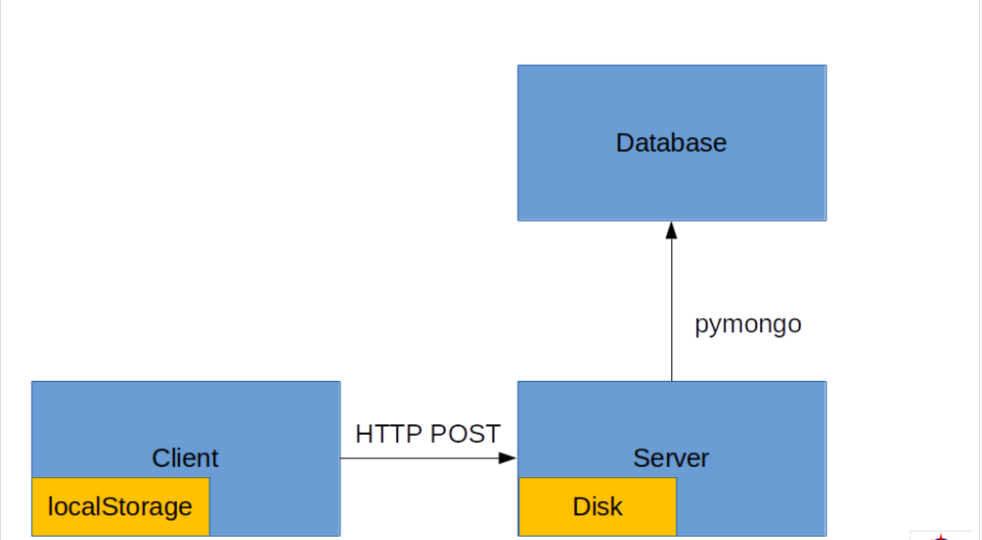
\includegraphics[width=60mm,scale=0.6]{HLD.png}
  \caption{High Level Design}
  \label{fig:HLDD}
\end{figure}
\section{Design Approach}
Here are two methodologies for software designing: 
\begin{itemize}
\item Top-down Design:It takes the entire programming framework as one entity and after that disintegrates it to accomplish in excess of one subsystem or some components based on few attributes.
\item Bottom-up Design: The model begins with most particular and essential components. It accedes with making more elevated amount out of subsystems by utilizing essential or lower level 
components.
\end{itemize}
As mentioned above the project requires two main modules to be implemented. Each module has its own components to be developed. We use bottom-up design strategy in this product design phase as we start designing the basic components in each module and finally we interlink both the modules to get the final product.

\section{System Architecture}
The architecture diagram design outline gives a review of a whole framework, distinguishing the 
primary segments that would be created for the item and their interfaces.
\begin{figure}[h!]
\centering
  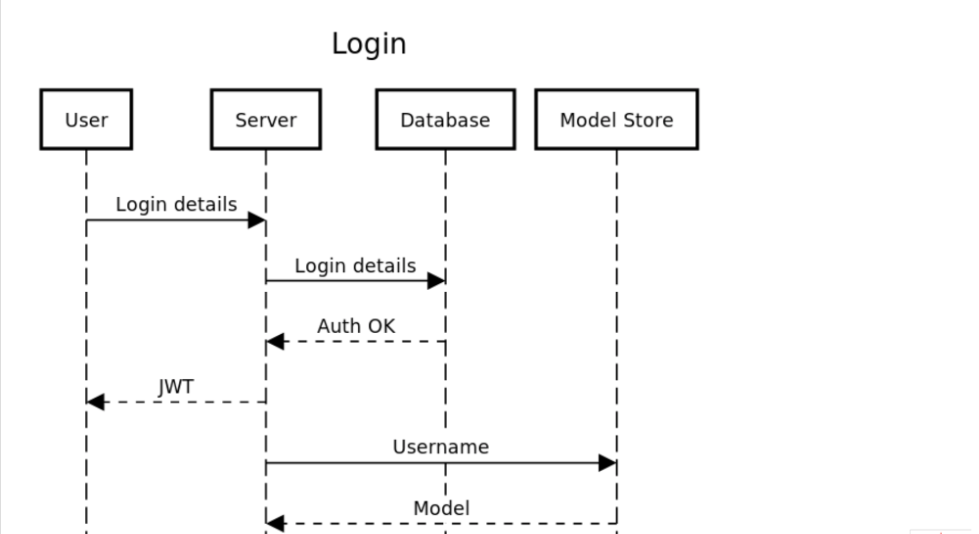
\includegraphics[width=\linewidth,scale=0.7]{login.png}
  \caption{System Architecture}
  \label{fig:Architecture}
\end{figure}
\pagebreak
\section{Sequence Diagram}
A sequence diagram is the representation of interactions of components among each
other in order. It shows the interactions between the objects in the system with the time order
that particular interaction takes place. Since it shows the time order of the interactions it is
called as sequence of events and hence the sequence diagram.
%\pagebreak

\begin{figure}[h!]
\centering
  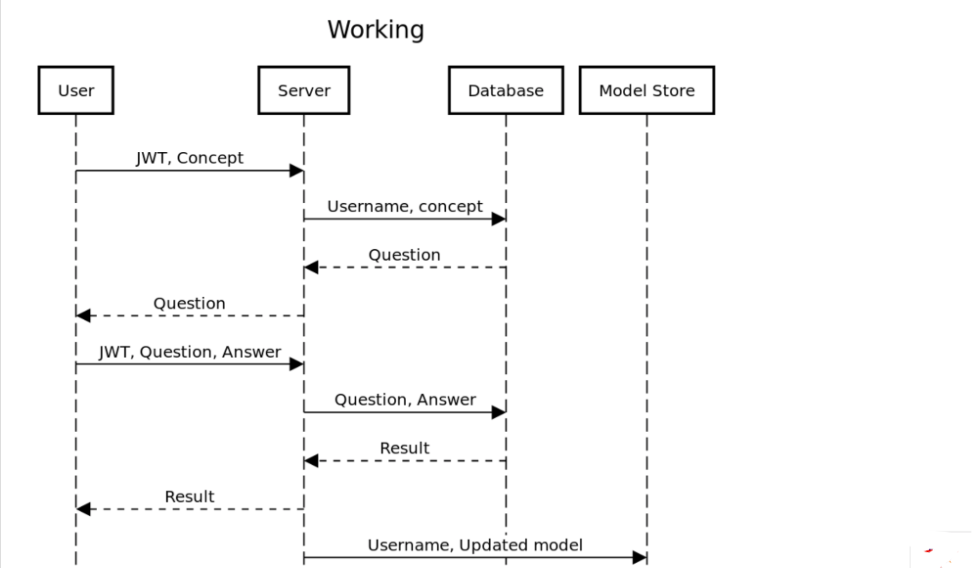
\includegraphics[width=100mm,scale=0.6]{Working.png}
  \caption{Sequence Diagram}
  \label{fig:Sequence}
\end{figure}
\pagebreak 
\section{Summary}
In this chapter we discussed the different design patterns which can be used in any product development cycle. For our project mainly sequence diagram is used. We also discussed the flowchart which shows the data flow between various components. This chapter even described the high level design.

\begin{thebibliography}{9}
\bibitem{p1} C. Piech, J. Bassen, J. Huang, S. Ganguli, M. Sahami, L. J. Guibas, and J. Sohl-Dickstein, (2015)
		\newblock Deep knowledge tracing
		\newblock \emph{Advances in Neural Information Processing Systems,} 505 -- 513.
		
		\bibitem{p1} C. Lin and M. Chi (2017)
		\newblock A comparisons of bkt, rnn and lstm for learning gain prediction
		\newblock \emph{International Conference on Artificial Intelligence in Education,} 536 -- 539, Springer.
		
		\bibitem{p1} Z. C. Lipton, D. C. Kale, C. Elkan, and R. Wetzel (2015)
		\newblock Learning to diagnose with lstm recurrent neural networks
		\newblock \emph{arXiv preprint,} arXiv:1511.03677.
		
		\bibitem{p1} J. Johns and B. Woolf (2006)
		\newblock A dynamic mixture model to detect student motivation and proficiency
		\newblock \emph{Proceedings of the National Conference on Artificial Intelligence,} 21(1), 163, AAAI Press; MIT Press.
		\bibitem{p1} A. T. Corbett and J. R. Anderson (1994)
		\newblock Knowledge tracing: Modeling the acquisition of procedural knowledge
		\newblock \emph{User modeling and user-adapted interaction,} 4(4), 253 -- 278.
		
		\bibitem{p1} R. S. d Baker, A. T. Corbett, and V. Aleven (2008)
		\newblock More accurate student modeling through contextual estimation of slip and guess probabilities in bayesian knowledge tracing
		\newblock \emph{Intelligent Tutoring Systems,} 253 -- 278, Springer.
		
		\bibitem{p1} C. Lin and M. Chi (2016)
		\newblock Intervention-bkt: incorporating instructional interventions into bayesian knowledge tracing
		\newblock \emph{International Conference on Intelligent Tutoring Systems,} 208 -- 218, Springer.
		
		\bibitem{p1} S. Chiappa and S. Bengio (2003)
		\newblock Hmm and iohmm modeling of eeg rhythms
for asynchronous bci systems
		\newblock \emph{Tech. rep.,} IDIAP.
		\bibitem{p1} S. Spaulding, G. Gordon, and C. Breazeal (2016)
		\newblock Affect-aware student models for robot tutors
		\newblock \emph{Proceedings of the 2016 International Conference on Autonomous Agents \& Multiagent Systems,} 864 -- 872, International
Foundation for Autonomous Agents and Multiagent Systems.
		
		\bibitem{p1} S. Schultz and I. Arroyo (2014)
		\newblock Tracing knowledge and engagement in parallel in an intelligent tutoring system
		\newblock \emph{Educational Data Mining}.
		
		\bibitem{p1} Z. A. Pardos and N. T. Heffernan (2011)
		\newblock Kt-idem: introducing item difficulty to the knowledge tracing model
		\newblock \emph{International Conference on User Modeling, Adaptation, and Personalization,} 243 -- 254, Springer.
		
		\bibitem{p1} M. V. Yudelson, K. R. Koedinger, and G. J. Gordon (2013)
		\newblock Individualized bayesian knowledge tracing models
		\newblock \emph{International Conference on Artificial Intelligence in Education,} 171 -- 180, Springer.
\end{thebibliography}
\rhead{\textit{Bibliography}}
\end{document}